% 本科毕业论文选项
\documentclass[bachelor,fandolfonts,replaceperiod]{jnuthesis} %Font: winfonts, sourcefonts, adobefonts.% now I replace adobefonts with fandolfonts
%\input{bachelor-common}
%\usepackage[math]{blindtext}
\usepackage[version=4]{mhchem}
\usepackage{zhlipsum}
\usepackage{lipsum}
%\usepackage{subfigure}
%\graphicspath{{Figure/}}
\titlea{含硒表面活性剂囊泡的构筑}
\titleb{与性质研究}
\author{陈育明}
\studentnum{1050115220}
\supervisor{刘雪锋}
\supervisorpos{教授}
\supervisorb{}
\supervisorbpos{}
\major{应用化学}
\department{化学与材料工程}
\institute{江南大学}
% 学士学位获得日期,需设置年、月,默认为编译日期。
\bachelordegreeyear{2019}
\bachelordegreemonth{6}

\begin{document}
    % 制作中文封面
    \maketitle
    % 开始前言部分
    \frontmatter
    % 论文的中文摘要
    \begin{abstract}
        复杂网络的研究可上溯到20世纪60年代对ER网络的研究。90年后代随着Internet
        的发展,以及对人类社会、通信网络、生物网络、社交网络等各领域研究的深入,
        发现了小世界网络和无尺度现象等普适现象与方法。对复杂网络的定性定量的科
        学理解和分析,已成为如今网络时代科学研究的一个重点课题。
        \keywords{开关表面活性剂;硒;氧化还原;囊泡}
    \end{abstract}
    
    % 论文的英文摘要
    \begin{englishabstract}
        \lipsum[1-2]
        % 英文关键词。关键词之间用英文半角逗号隔开,末尾无符号。
        \englishkeywords{Switchable Surfactant, Selenium, Redox, Vesicle}
    \end{englishabstract}
    
    % 生成论文目次
    \tableofcontents
    
    % 开始正文部分
    \mainmatter
    
    \chapter{绪论}\label{chapter:introduction}
    \section{引言}
    
    【表面活性剂简述】表面活性剂因其乳化、润湿、增溶等优良作用而广泛应用于诸如原油回收、
    土壤修复、乳液聚合、药物制备等领域\cite{秦勇2009}。
    
    一般情况下,表面活性剂大多具有性能稳定的特点,但在    大多数情况下,它只在某一阶段起作用,
    过程结束后,往往分离困难,另一方面,表面活性剂一般不参与化学反应,直接排放既是一种浪费,
    同时给环境带来压力\cite{秦勇2009}。因此,人们先后发展了多样触发机制的的可分解表面活性剂 (Cleavable Surfactants)
    和开关型表面活性剂 (Switchable Surfactants)。
    
    \section{开关型表面活性剂}
    为应对传统表面活性剂生物降解速率慢、引起的环境问题,人们开始关注于可分解表面活性剂,设想通过
    分子内嵌入易断裂化学键以提供生物降解速率(尽管化学研究中的高效催化分解未必能够体现完全在实际中的微生物高效降解),此类表面活性剂在酸、碱、光照、加热、酶催化等
    条件下能够促发分解\cite{hellberg2000}。
    
 可分解表面活性剂最初主要是为了
    解决环境问题而发展起来的,理论设想通过在分子中嵌入
    易断裂化学键提高生物降解速率,尽管研究中所发现的高效酶催化或化学催化分解未必
    总能够反映到实际中微生物的高效降解\cite{tehrani2007}。传统表面活性剂一般相对稳定,
    早在可分解表面活性剂概念发展之前,季铵酯类表面活性剂已用作纺织品柔软剂,其便是典型的
    可分解表面活性剂。此外,十二烷基硫酸钠的自催化降解、脂肪酸聚氧乙烯酯应当在中性或
    弱碱性使用、羰基表面活性剂酸性条件可分解均被人们注意并用以实际\cite{tehrani2007}。
    
    而对于可分解表面活性剂,其可采用酶催化分解,也可采用酸催化、碱催化水解或是UV光照、
    臭氧以及加热等手段进行分解,可分解表面活性剂主要包含对酸不稳定(缩醛类、缩酮类、
    原酸酯类及硅氧烷基表面活性剂)、对碱不稳定(季铵酯、甜菜碱酯、单烷基(醚)碳酸酯)以及
    对UV-光照、热及臭氧不稳定的各类表面活性剂\cite{hellberg2000,tehrani2007,shukla2010,narayanan2008}。%,相关文献\cite{hellberg2000,tehrani2007,shukla2010,narayanan2008}对此
    %进行了综述,各类型代表可分解表面活性剂见图\ref{fig:cleavable-saa} or 图\ref{fig:cleavable-a}。
    
    %    \begin{figure}
    %        \centering
    %        \subfloat[][]{%
    %        \label{fig:cleavable-a}%
    %        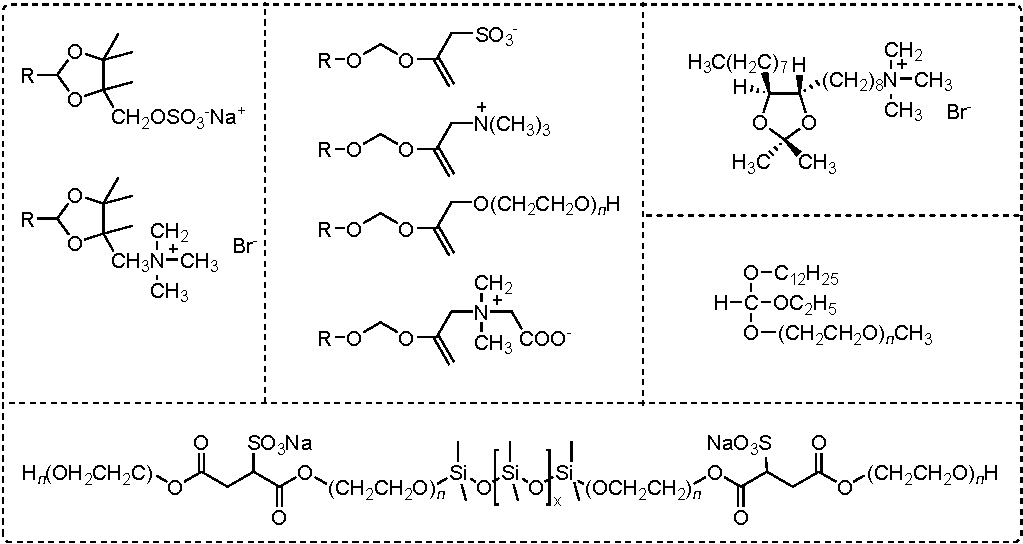
\includegraphics[width=.9\textwidth]{Figure/cleavable-a.png}}%
    %        %\hspace{8pt}%
    %        \subfloat[][]{%
    %        \label{fig:ex3-b}%
    %        \includegraphics[width=.9\textwidth]{example-image}}\\
    %        \subfloat[][]{%
    %        \label{fig:ex3-c}%
    %        \includegraphics[width=.9\textwidth]{example-image}}%
    %       % \hspace{8pt}%
    %        \subfloat[][]{%
    %        \label{fig:ex3-d}%
    %        \includegraphics[width=.9\textwidth]{example-image}}%
    %        \caption[A set of four sub-floats.]{A set of four sub-floats:
    %        \subref{fig:cleavable-a} 对酸性不稳定的可分解表面活性剂;
    %        \subref{fig:ex3-b} describes the second sub-float;
    %        \subref{fig:ex3-c} describes the third sub-float; and,
    %        \subref{fig:ex3-d} describes the last sub-float.}%
    %        \label{fig:ex3}%
    %    \end{figure}
    
    %    \begin{figure}
    %        \centering
    %        \begin{subfigure}[b]{\textwidth}
    %            \centering
    %            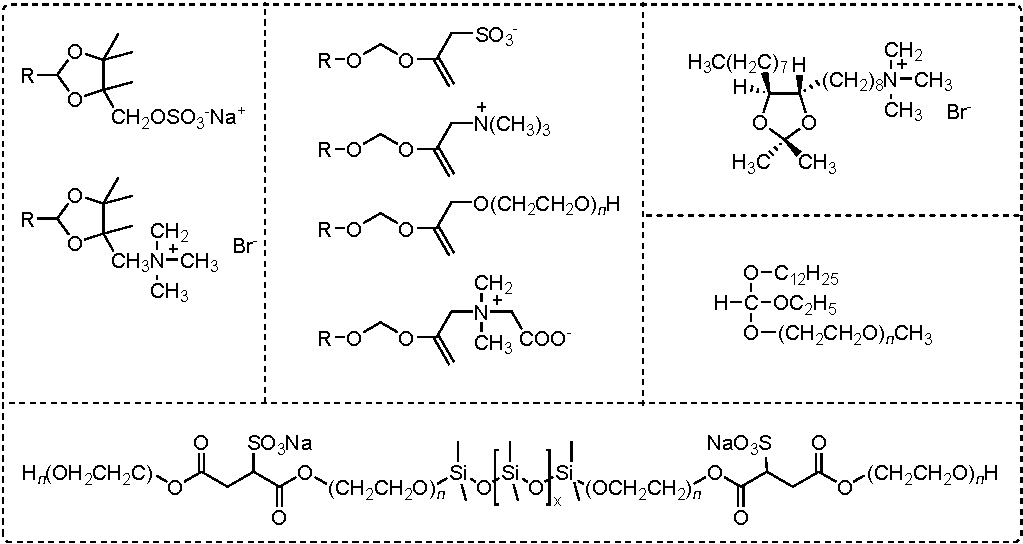
\includegraphics[width=\textwidth]{Figure/cleavable-a.pdf}
    %            \caption{对酸性不稳定的可分解表面活性剂}\label{fig:cleavable-a}
    %        \end{subfigure}%
    %    
    %        \begin{subfigure}[b]{\textwidth}
    %            \centering
    %            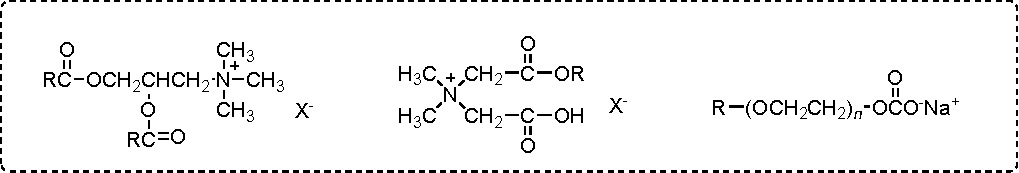
\includegraphics[width=\textwidth]{Figure/cleavable-b.pdf}
    %            \caption{对碱性不稳定的可分解表面活性剂}\label{fig:cleavable-b}
    %        \end{subfigure}
    %    
    %        \begin{subfigure}[b]{\textwidth}
    %            \centering
    %            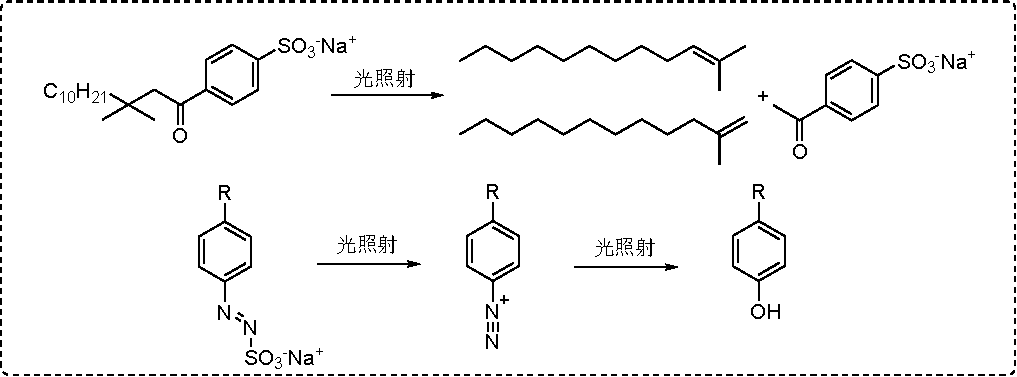
\includegraphics[width=\textwidth]{Figure/cleavable-c.pdf}
    %            \caption{光照分解表面活性剂}\label{fig:cleavable-c}
    %        \end{subfigure}%
    %
    %        \begin{subfigure}[b]{\textwidth}
    %            \centering
    %            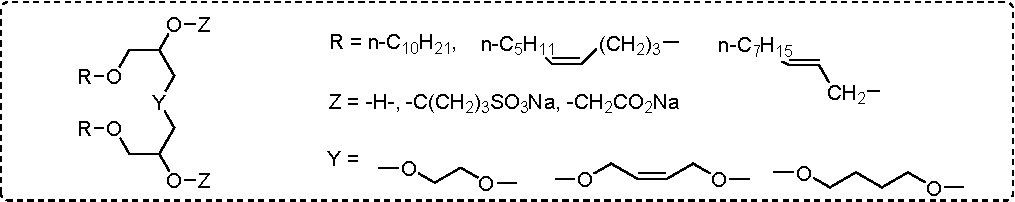
\includegraphics[width=\textwidth]{Figure/cleavable-d.pdf}
    %            \caption{臭氧分解表面活性剂}\label{fig:cleavable-d}
    %        \end{subfigure}
    %    \end{figure}
    %%\addtocounter{figure}{-1} % 将图的编号减1
    %\begin{figure}[t]
    %%\addtocounter{subfigure}{1} % 子图编号加2
    %        \begin{subfigure}[b]{\textwidth}
    %            \centering
    %            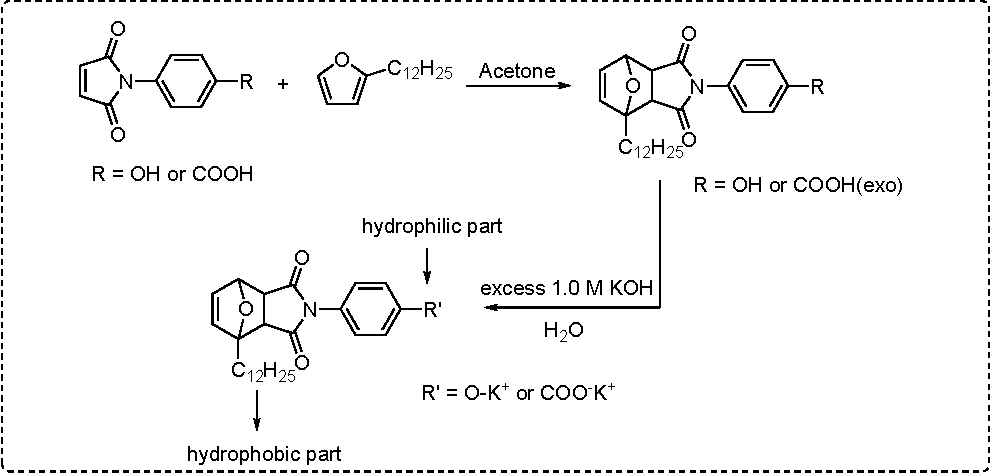
\includegraphics[width=\textwidth]{Figure/cleavable-e.pdf}
    %            \caption{臭氧分解表面活性剂}\label{fig:cleavable-e}
    %        \end{subfigure}
    %        \caption{已发展的可分解表面活性剂类型}\label{fig:cleavable-saa}
    %    \end{figure}
    %    e. 通过Diels-Alder反应合成的热不稳定可分解表面活性剂
    
        可分解表面活性剂发展的最初目的是为了解决传统表面活性剂难生物降解的环境问题,同时
    可分解表面活性剂也可在乳化阶段之后通过刺激手段使乳液破乳,也可用于纳米粒子及聚合物制备中
    易脱除的模板剂\cite{liu2007}。此外,一些研究将分解表面活性剂用于膜蛋白的质谱分析\cite{norris2003}
    及胶束电动色谱\cite{stanley2012}。但与此同时,化学或酶催化降解有时不能完全适合于微生物的
    降解\cite{tehrani2007},或是降解速率不高,更重要的一点是其分解过程不可逆\cite{liu2007}。
    
    可分解表面活性剂研究较早,最主要面向解决传统表面活性剂的生物降解问题,已有PPS、ProteaseMAX、
    RapiGest SF等商品化洗涤产品应用可分解表面活性剂。此外,可分解表面活性剂在生物化学、
    医药制造等领域也可有所应用\cite{hellberg2000}。Liu等\cite{guo2012}以氯化肉豆蔻酰胆碱
    (及一种季铵酯表面活性剂,在酶催化或碱催化下可分解)及对磺酸杯芳烃(SC4A)构建二级囊泡,
    利用氯化肉豆蔻酰胆碱在丁酰胆碱酯酶(BChE)作用下酯键断裂,或可应用于阿尔茨海默症的载药及释放(见图\ref{fig:Ch1-SC4A})。
    
    \begin{figure}[htbp]
        \centering
        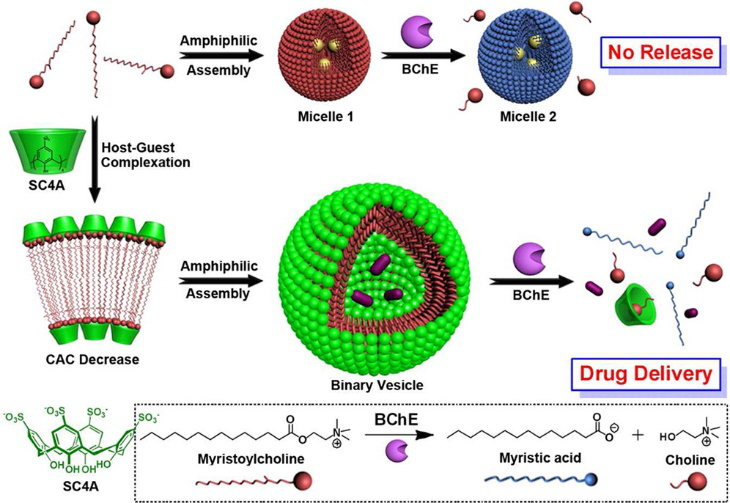
\includegraphics[width= 0.55\textwidth]{Figure/Ch1-SC4A}\\
        \caption{肉豆蔻酰胆碱在SC4A空白及存在下的两亲自组装示意图}\label{fig:cleavale-SC4A}
    \end{figure}
    
   【转向开关表活】
    
    20世纪80年代
    以来,各种触发机制的开关表面活性剂(Switchable Surfactants)被发展出来,用于调控
    表面活性剂性质,例如,聚合物的乳胶悬浮液在储存运输中需要是稳定的,担当其被施工涂到
    表面之后并不需要稳定的悬浮液,那么能够对这一性质进行“关闭”显然是此类表面活性剂的
    有点\cite{jessop2012}。同时,开关表面活性剂这种“关闭”是可以通过另一种手段进行恢复的。
    本文将简述可分解表面活性剂及其应用的概况,并就刺激手段为分类方式概述开关表面活性剂的发展状况。
    
    相比可分解表面活性剂分解不可恢复,开关表面活性剂的性质转变是可逆的,是可以调控的,
    例如,非离子表面活性剂就是一类传统的温度开关表面活性剂,当温度上升,其亲水性降低、
    表面活性降低,当温度恢复时其性质亦恢复。根据这些刺激响应的方式,可将开关表面活性剂分为:
    光开关、磁开关、温度开关、酸碱开关、\ce{CO2}开关及包含电化学方法和化学方法的氧化-还原开关表面活性剂\cite{秦勇2009}。
    
    \subsection*{(1) 光开关表面活性剂}
    光开关表面活性剂在非极性疏水尾链或极性亲水头基中具有适当的显色基团\cite{张冤帝2017}。
    根据所需光照条件可将光开关表面活性剂分为两类:一类时热稳定型的,利用不同波长的光可
    调节表面活性剂的表面活性;另一类是不稳定的,只有用连续光照才可实现表面活性的转变。
    根据表面活性剂分子在转变中的变化特点,可将光开关表面活性剂分为顺反异构型、裂解-聚合型以及
    极性变化型开关表面活性\cite{张冤帝2017,李云霞2011}。
    顺反异构型开关表面活性剂是研究较早的光开关表面活性剂,其主要其结构有偶氮苯类、
    二苯乙烯类及烷基苯乙烯衍生物,此外,还有一些异构型光开关表面活性剂。异构型光开关表面活性剂
    见图\ref{fig:switchable-light}\cite{张冤帝2017,karthaus1996,shang2003,吕湘亮2018}。
    
    \begin{figure}[htbp]
        \centering
        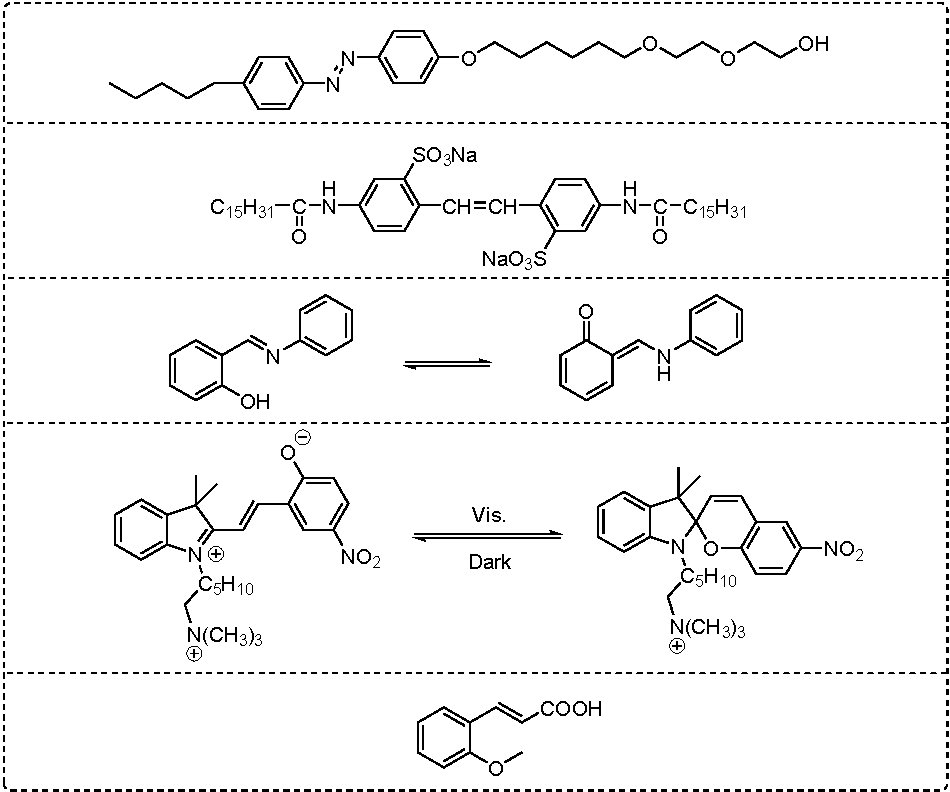
\includegraphics[width= \textwidth]{Figure/switchable-light.pdf}\\
        \caption{电化学方法实现氧化-还原开关表面活性剂:二茂铁基和联吡啶类开关表面活性剂}\label{fig:switchable-light}
    \end{figure}
    
    图\ref{fig:switchable-light} 几类异构型光开关表面活性剂\cite{张冤帝2017,karthaus1996,shang2003,吕湘亮2018}
    其中,偶氮型光开关表面活性剂研究较早,应用较广,一些光敏表面活性剂如偶氮类分解型及
    光照不可逆型不当归入光开关表面活性剂,刘清斌在其硕士论文中对光敏型表面活性剂做了总结\cite{刘清斌2018}。
    光开关表面活性剂或可在生物医药、环境修复及减阻传热等方面有所应用\cite{刘清斌2018},
    偶氮类光致异构化表面活性剂研究较多,我校王潮霞课题组\cite{chen2016}采用偶氮类阳离子表面活性剂BTAEAzo的光刺激开关实现绿色化的泡沫染整工艺。
    
    图 4 偶氮苯类阳离子表面活性剂的光致异构化\cite{chen2016}
    除光开关表面活性剂自生结构变化外,还可使用光相应分子与表面活性剂复配,构建光刺激相应系统,
    Zhao等\cite{zhao2016}将反式-邻甲氧基肉桂酸与N-甲基-N-乙基吡咯烷溴化物(C16MPB)碱性条件下
    自组装成为粘弹性蠕虫状胶束,经UV光照后反式-邻甲氧基肉桂酸构型转变,使体系转变成球形或棒状胶束。
    
    图 5 N-甲基-N-乙基吡咯烷溴化物(C16MPB)与邻甲氧基肉桂酸构成的光刺激响应体系\cite{zhao2016}。
    
    \subsection*{(2) 磁开关表面活性剂}
    磁开关表面活性剂含有磁响应结构,有离子液体、螯合型以及多金属氧酸盐表面活性剂,此外,
    磁性有机分子表面活性剂是有待发展的新一类磁表面活性剂\cite{brown2015},Brown\cite{brown2015}对此类
    磁表面活性剂进行了综述,磁响应表面活性剂可用于蛋白质分离、水处理以及环境修复\cite{brown2015}。
    几类磁相应表面活性剂见图 6。
    
    图 6 三类主要的磁表面活性剂及一类潜在的磁表面活性剂\cite{brown2015,brown2012}
    
    \subsection*{(3) 温度开关表面活性剂}
    非离子型表面活性剂是典型的温度开关表面活性剂,随温度升高其亲水性会逐渐下降,
    至浊点时亲水性显著降低,表面活性变差,而当温度降低后其又可恢复表面活性。Chu\cite{chu2011}等
    以PDAS为表面活性剂制备了一种温度响应凝胶,在30℃时形成球状或短棒状胶束,在40℃时则形成
    网络蠕虫状胶束,这是由于加热时疏水部分溶解度降低,从而形成网状交联凝胶。
    
    图 7 可切换温感凝胶
    \subsection*{(4) 酸碱开关表面活性剂}
    酸碱开关表面活性剂即pH 开关表面活性剂,其通常含有羧酸、脒基、胍基等酸性或碱性基团,
    在pH 变化时,这些基团接受或给予质子,导致表面活性剂亲水或疏水性发生变化,从而调控
    表面活性剂的表面活性\cite{吕湘亮2018}。Lv\cite{lv2014}等合成一类酸碱开关Gemini表面活性剂,
    通过调控pH可实现制备的乳液在O/W乳液“开启”和W/O乳液“关闭”之间反转,见图 8。
    
    图 8 pH开关表面活性剂控制乳液类型转变
    此外,除通过pH调节表面活性剂亲疏水性改变体系性质,Brazdova\cite{李云霞2011,brazdova2008}等
    制得脂质体表面活性剂,通过pH 控制物质构象转化作为开关,见图 9。
    
    图 9 pH调节构象作为开关
    \subsection*{(5) \ce{CO2}/\ce{N2}开关表面活性剂}
    \ce{CO2}型开关表面活性剂其作用原理本质上和酸碱开关表面活性剂类似,利用\ce{CO2}气体的弱酸性,
    随着\ce{CO2}的通入和排出,体系的pH发生变化,从而引起体系内可离子化基团质子化或去质子化,
    导致亲疏水性发生变化,进而影响体系的表面活性。迄今为止,\ce{CO2}开关型表面活性剂主要包括
    脒/\ce{CO2}体系、胍/\ce{CO2}体系以及胺/\ce{CO2}体系\cite{梅平2016}。
    \ce{CO2}型开关表面活性剂采用\ce{CO2}作为调控手段,相比其他调控手段,价格便宜、无毒害且易除去等
    优点\cite{jessop2012},可应用于重油输送、土壤清洗、油砂分离及乳化聚合\cite{jessop2012}。
    早在开关表面活性剂概念提出之前,\ce{CO2}型开关表面活性剂已投入使用,Moore和Lefevre采用\ce{CO2}作为
    丁二烯/苯乙烯乳液聚合的开关表面能活性剂(见图 10.a),其中左式具有乳化作用而右式不具有乳化作用。
    
    图 10 较早应用及研究的\ce{CO2}型开关表面活性剂
    
    2006年,Jessop课题组\cite{liu2006science}提出一类脒类化合物可用于\ce{CO2}开关表面活性剂,
    此外,三级胺也可用于\ce{CO2}开关表面活性剂,但一级、二级胺则因为形成氨基甲酸酯在开关
    表面活性剂应用中有所难度\cite{jessop2012}。
    \subsection*{(6) 氧化-还原开关表面活性剂}
    氧化还原型开关表面活性剂采用电化学方法或化学手段改变表面活性剂分子内部分结构,
    从而达到调整表面活性的目的。其中,前者研究最早且较为成熟的是二茂铁基表面活性剂
    ,其包含阳离子-两性离子可逆转换和阴离子-两性离子可逆转换两类\cite{李云霞2011}。
    图\ref{fig:switchable-redox-cp2fe}中前者是一类二茂铁基表面活性剂。但二茂铁基开关表面活性剂所需使用的二茂铁基团
    价格对该类表面活性剂的使用有所限制。
    
    \begin{figure}[htbp]
        \centering
        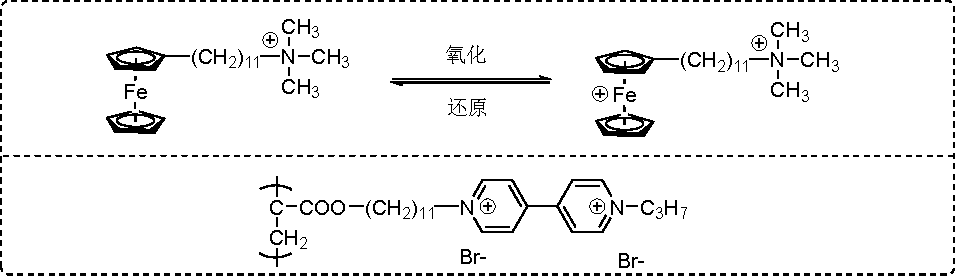
\includegraphics[width= \textwidth]{Figure/switchable-cp2fe.pdf}\\
        \caption{电化学方法实现氧化-还原开关表面活性剂:二茂铁基和联吡啶类开关表面活性剂}\label{fig:switchable-redox-cp2fe}
    \end{figure}
    
    此外,甲基紫类结构,即联吡啶类结构的表面活性剂也是一类良好的氧化-还原表面活性剂,
    但此类表面活性剂具有高毒性,如氯化二甲基联吡啶(即百草枯主要成分,一种高度植物农药)。
    
    除以上电化学方法的氧化还原表面活性剂之外,含二硫键结构的表面活性剂可在如含巯基试剂作用下断裂,
    从而改变分子结构。
    
    图 12 二硫键型氧化-还原开关表面活性剂
    最后,含硒表面活性剂作为一种新型的氧化-还原开关表面活性剂,Kong等\cite{kong2016redox}利用
    \ce{H2O2}将硒醚氧化为硒亚砜,使尾链亲水性增加,且在\ce{Na2SO3}等还原条件下又可恢复原结构。
    
    图 13 含硒氧化-还原表面活性剂的可逆转化\cite{kong2016redox}
    
    \subsection*{(7) 酶开关表面活性剂}
    除以上类型的开关表面活性剂之外,还有酶催化\cite{ku2011}【Enzyme-triggered model self-assembly in surfactant–cyclodextrin systems】的开关表面活性剂有待讨论。
    
    
    \section{含硒表面活性剂}
    \zhlipsum[1]
    
    \section{囊泡}
    \zhlipsum[1]
    
    \section{论文的目的与创新}
    \subsection{研究目的}
    \zhlipsum[1]
    \subsection{创新之处}
    \zhlipsum[1]
    \subsection{研究内容}
    \zhlipsum[1]
    
    %%%%%%%%%%%%%%%%%%%%%%%%%%%%%%%%%%%%%%%%%%%%%%%%%%%%%%%%%%%%%%%%%%%%%%%%%%%%%%%
    \chapter{实验部分}\label{chapter:experiment}
    \section{实验仪器与试剂}
        \begin{table}[htp]
        \centering
        \begin{tabular}{ccc}
            \toprule
            \textbf{仪器/试剂} & \textbf{规格/型号} & \textbf{生产厂家} \\
            \midrule
            硒   &  RG  & 阿达玛斯试剂 \\
s          硼氢化钠  & AR  & 上海化学试剂有限公司 \\
            1-溴代十二烷  & CP & 国药集团化学试剂有限公司 \\
            3-溴丙醇 & java.math.和具体值有关 & 国药集团化学试剂有限公司 \\
            氯磺酸  & java.math.B值有关 & 国药集团化学试剂有限公司 \\
            硫酸钠  & java.math.B值有关 & 国药集团化学试剂有限公司 \\
            亚硫酸钠  & java.math.B值有关 & 国药集团化学试剂有限公司 \\
            旋转蒸发器  & java.math.B值有关 & 国药集团化学试剂有限公司 \\
            超声波清洗器  & java.math.B值有关 & 国药集团化学试剂有限公司 \\
            核磁共振谱仪  & java.math.B值有关 & 国药集团化学试剂有限公司 \\
            双氧水  & java.math.B值有关 & 国药集团化学试剂有限公司 \\
            电子分析天平  & java.math.B值有关 & 国药集团化学试剂有限公司 \\
            液相色谱质谱联用仪  & java.math.B值有关 & 国药集团化学试剂有限公司 \\
            超级恒温水浴  & java.math.B值有关 & 国药集团化学试剂有限公司 \\
            \bottomrule
        \end{tabular}
        \caption{实验仪器与试剂}\label{table:实验仪器与试剂}
    \end{table}

    \zhlipsum[1]
    
    \section{含硒表面活性剂的制备}
    \subsection{含硒表面活性剂的合成路线}
    \begin{figure}[htbp]
        \centering
        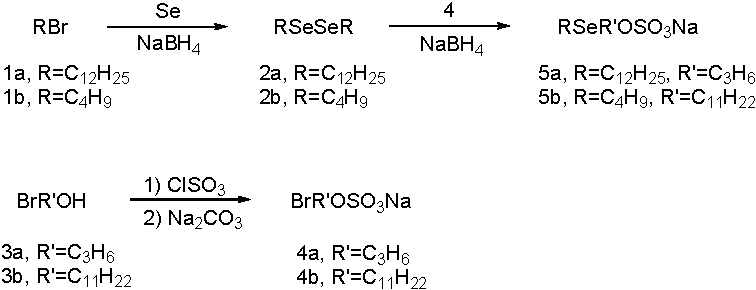
\includegraphics[]{Figure/synthesis.pdf}\\
        \caption{含硒表面活性剂的合成路线}\label{fig:synthesis}
    \end{figure}
    
    \zhlipsum[1]
    
    \section{囊泡的构筑}
    \zhlipsum[1]
    
    \section{囊泡的性质研究}
    \subsection{不同摩尔比}
    
    \subsection{稳定性}
    
    \subsection{不同浓度}
    
    \subsection{氧化还原响应}
    
    \begin{definition}[平均路径长度]
        网络的平均路径长度$L$定义为任意两个节点之间的距离的平均值,即
        \begin{equation}\label{eq:avarage_path_lentgh}
        L = \frac{2}{N(N+1)}\sum_{i\geq j}d_{ij}
        \end{equation}
        其中$N$为网络节点数。网络的平均路径长度也称为网络的特征路径长度。
    \end{definition}
    
   %%%%%%%%%%%%%%%%%%%%%%%%%%%%%%%%%%%%%%%%%%%%%%%%%%%%%%%%%%%%%%%%%%
    \chapter{实验结果与讨论}\label{chapter:results}
    \section{含硒表面活性剂的表征与分析}
    以\ce{CD3OD} (δ = 3.31)为溶剂,其中含有少量的\ce{H2O} (δ = 4.87)\cite{babij2016nmr} ,对纯化后的样品进行
    \ce{^1H} NMR 表征,表征与分析结果如图\ref{fig:NMR-12+3}所示。
    \begin{figure}[htbp]
        \centering
        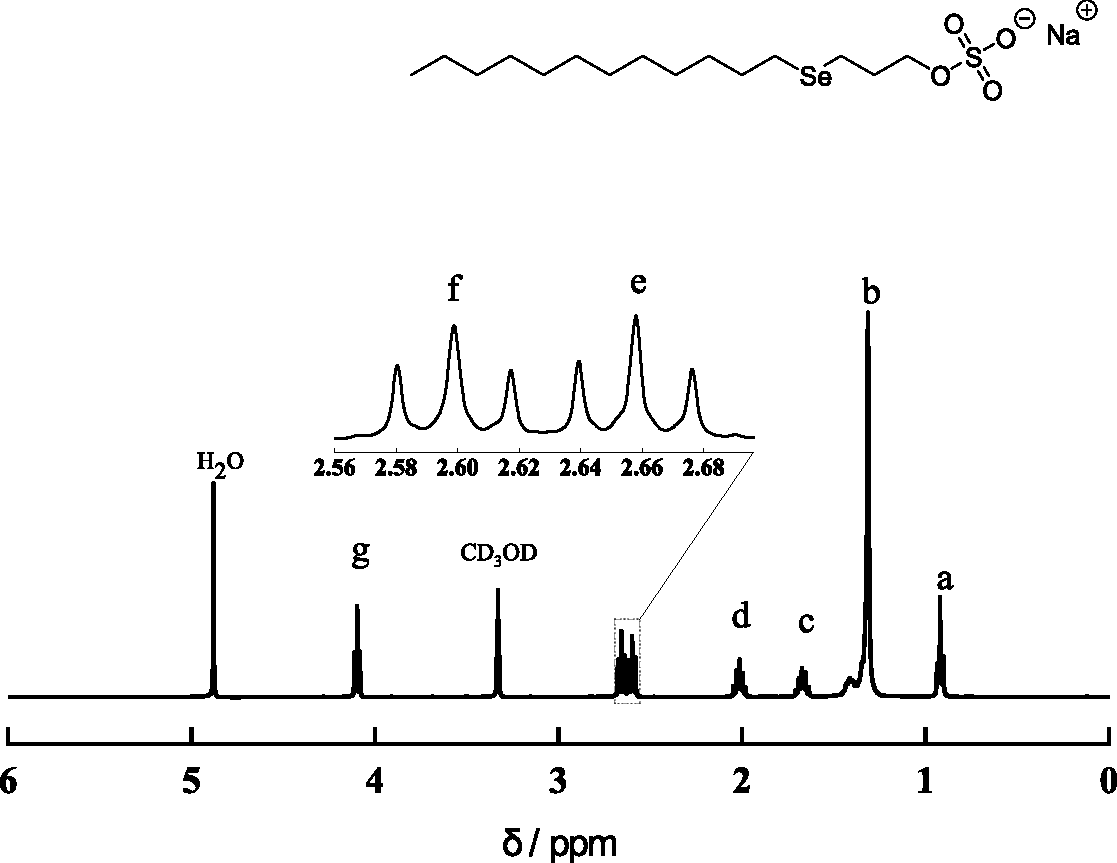
\includegraphics[width=.7\textwidth]{figure/nmr1232.pdf}\\
        \caption{核磁}\label{fig:NMR-12+3}
    \end{figure}
    
    对 \ce{C12SeAS} 的核磁共振氢谱进行解析,化学位移为 0.921 处的三重峰为 C 12 SeAS 疏水尾
    链端的甲基上的氢信号,以其积分个数为 3 计算,结果如表 2-5 所示,实际总氢个数为 31.68,
    理论氢个数为 31,氢个数基本吻合;如图 2-7 所示,e 处的两个三重峰氢信号为 Se 两端的亚
    甲基的氢信号,f 处亚甲基上的氢由于靠近极性头基(SO 4 - ),出峰位置移动到 4.097,各个氢信
    号的出峰位置与目标产物能够对应,由此推断检测样品即为目标产物。
    
    \begin{figure}[htbp]
    \centering
        \begin{subfigure}[b]{.475\textwidth}
            \centering
            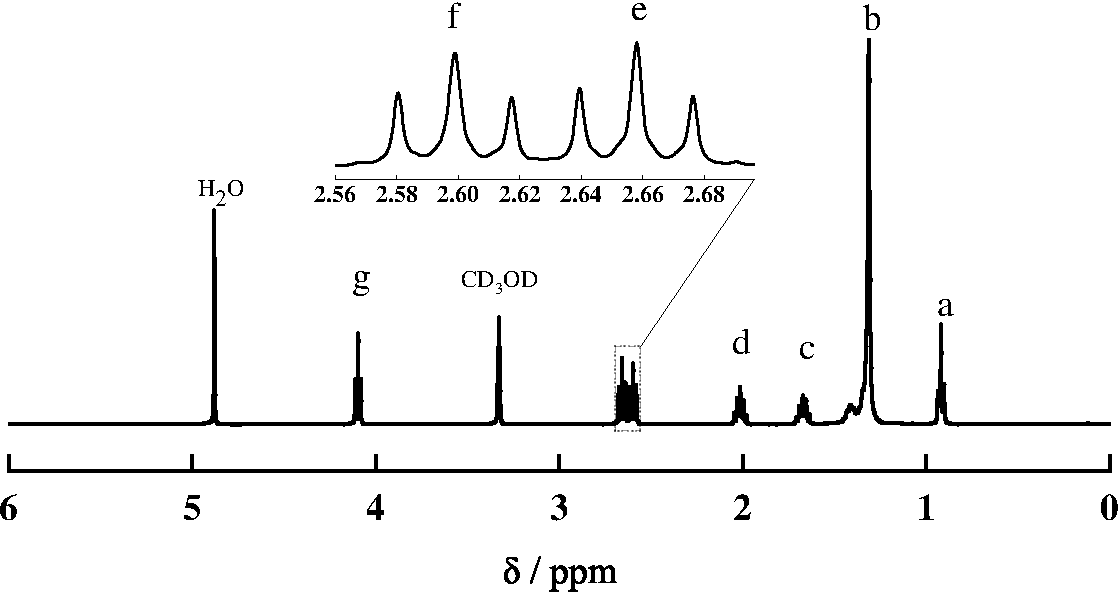
\includegraphics[width=\textwidth]{figure/nmr123.pdf}
            \caption{核磁}\label{}
        \end{subfigure}
        \hfill
        \begin{subfigure}[b]{.475\textwidth}
            \centering
            \includegraphics[width=\textwidth]{example-image}
            \caption{质谱}\label{}
        \end{subfigure}
    \caption{12+3结构表征}\label{fig:cleavable-saa}
    \end{figure}

    \begin{figure}[htbp]
        \centering
        \begin{subfigure}[b]{.475\textwidth}
            \centering
            \includegraphics[width=\textwidth]{example-image}
            \caption{核磁}\label{}
        \end{subfigure}
        \hfill
        \begin{subfigure}[b]{.475\textwidth}
            \centering
            \includegraphics[width=\textwidth]{example-image}
            \caption{质谱}\label{}
        \end{subfigure}
        \caption{4+11结构表征}\label{fig:cleavable-saa}
    \end{figure}
    
    \section{12+3复配囊泡的性质研究}
    \subsection{不同摩尔比复配}
    
    \subsection{囊泡稳定性}
    
    \subsection{不同浓度构筑含硒SAA囊泡}

    \begin{figure}[htbp]
        \centering
        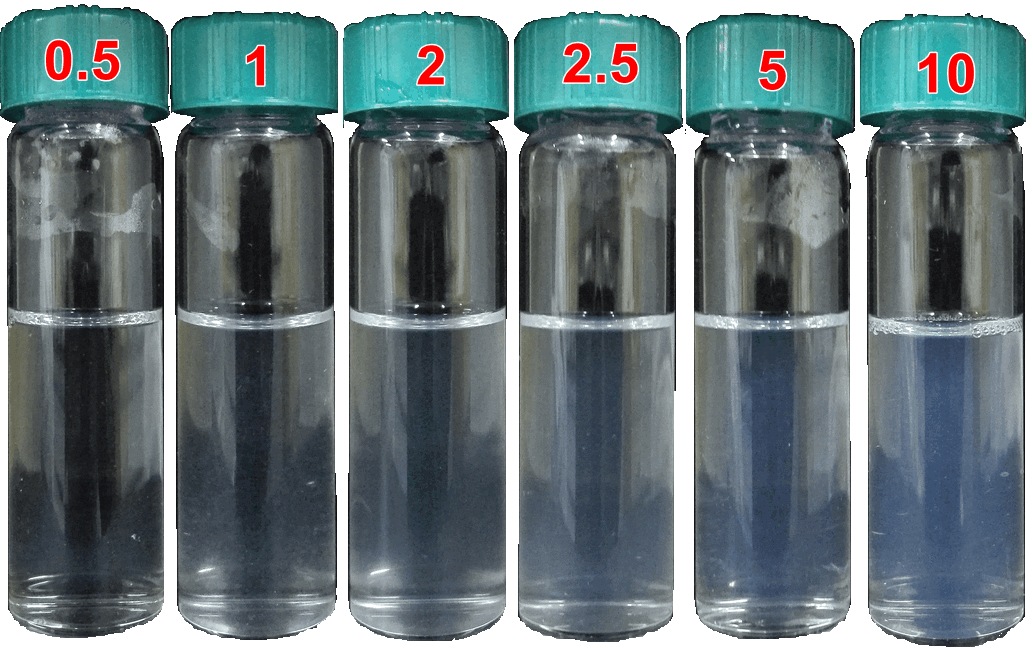
\includegraphics[height=4.5cm]{figure/123concentration.png}\\
        \caption{12+3不同浓度复配囊泡}\label{fig:vesicle-concentration}
    \end{figure}

    \begin{figure}[htbp]
        \centering
        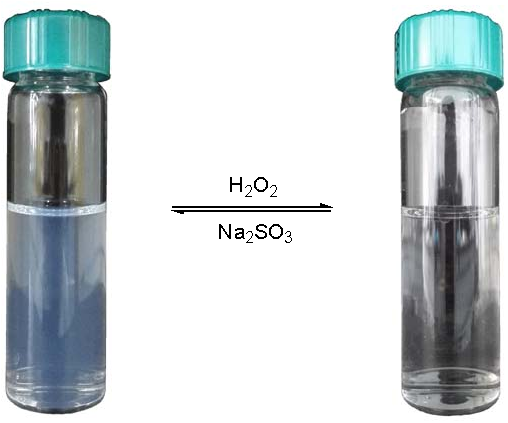
\includegraphics[height=4.5cm]{figure/redox.pdf}\\
        \caption{不同浓度复配囊泡}\label{fig:vesicle-redox}
    \end{figure}

    \subsection{氧化还原响应}
    
    
    [12+3]与DTAB复配囊泡
    
    \section{4+11复配囊泡的性质研究}
    \subsection{不同摩尔比复配}
    
    \subsection{囊泡稳定性}
    
    \subsection{不同浓度}
    \begin{figure}[htbp]
        \centering
        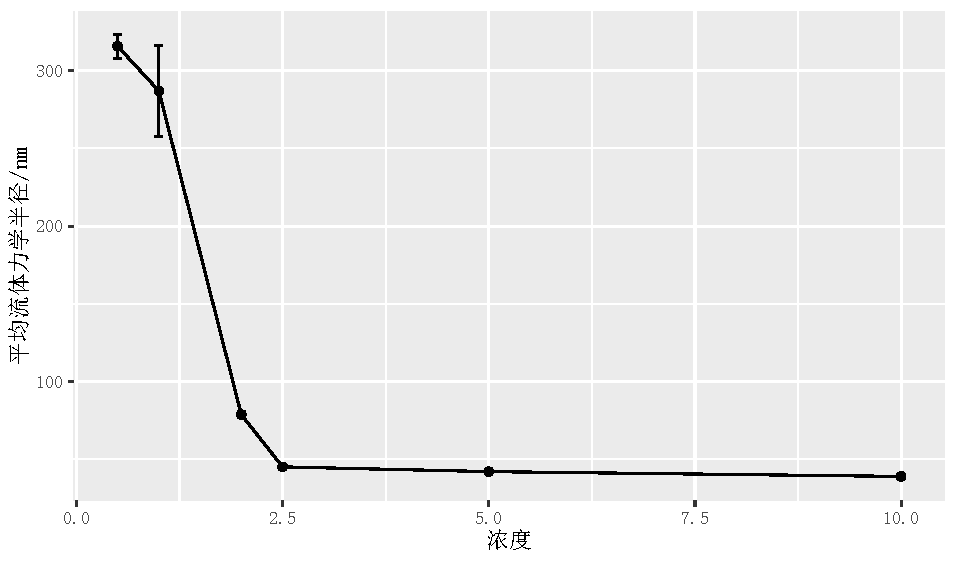
\includegraphics[width=0.8\linewidth]{Figure/test.pdf}\\
        \caption{4+11不同浓度复配囊泡}\label{fig:vesicle-concentration-line}
    \end{figure}
    \subsection{氧化还原响应}
    
    
    [一次还原稳定性]加入后立即
    \section{本章小结}

    %%%%%%%%%%%%%%%%%%%%%%%%%%%%%%%%%%%%%%%%%%%%%%%%%%%%%%%%%%%%%%%
    % 学位论文的正文应以《结论》作为最后一章
    \chapter{结论与展望}\label{chapter:concludes}
    \section{结论}
    本文在第\ref{chapter:experiment}章中,通过考虑数据中心网络布局构建中的最大度限制
    问题,提出了符合数据中心网络基本要求的DS小世界模型,并分析了它的性质。随后提出
    SIDN,将DS模型映射到具体的网络结构中,并分析了所构成网络的平均直径、网络总带宽、
    对故障的容错能力等各项网络性能。
    
    \zhlipsum[1-3]
    
    \section{不足之处及未来展望}
    在第\ref{chapter_experiments}章中,针对网络模型研究这一类工作的共性,设计构造通
    用验证平台系统。以海量虚拟机和虚拟分布式交换机的形式,实现了基于少量物理节点,对
    大规模节点的模拟。其模拟运行的过程与真实运行在实现层面完全一致,运行的结果与真实
    环境线性相关。除为本文所涉若干网络模型提供验证外,可进一步推广到更为广泛的领域,
    为各种网络模型及路由算法的研究工作,提供分析、指导与验证。
    
    \begin{backmatter}
    \fancyhead[C]{\songti\zihao{-5}参考文献}
    % 推荐使用BibTeX,若不使用BibTeX时注释掉下面一句。
    %\nocite{*}
    \bibliography{bachelor}
    \end{backmatter}

    %%%%%%%%%%%%%%%%%%%%%%%%%%%%%%%%%%%%%%%%%%%%%%%%%%%%%%%%%%%%%%%
    % 致谢,应放在《结论》之后
    \begin{acknowledgement}
        \fancyhead[C]{\songti\zihao{-5}致谢}
        首先感谢我的母亲韦春花对我的支持。其次感谢我的导师陈近南对我的精心指导和热心帮助。接下来,
        感谢我的师兄茅十八和风际中,他们阅读了我的论文草稿并提出了很有价值的修改建议。
        
        最后,感谢我亲爱的老婆们:双儿、苏荃、阿珂、沐剑屏、曾柔、建宁公主、方怡,感谢
        你们在生活上对我无微不至的关怀和照顾。我爱你们!
    \end{acknowledgement}
    
%    \begin{backmatter}
%    \fancyhead[C]{\songti\zihao{-5}附录}
%    \chapter{附录 A:彩色插图}
%    \begin{figure}[htbp]
%        \centering
%        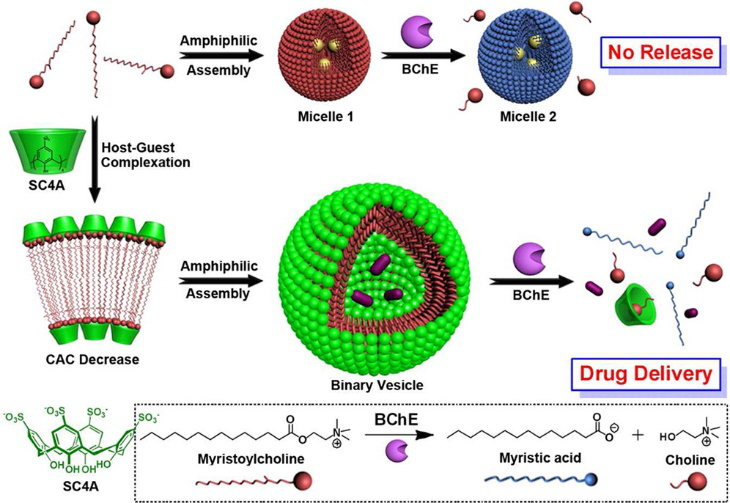
\includegraphics[width= 0.55\textwidth]{Figure/Ch1-SC4A}\\
%        \caption{肉豆蔻酰胆碱在SC4A空白及存在下的两亲自组装示意图}
%    \end{figure}
%    \end{backmatter}
    %%%%%%%%%%%%%%%%%%%%%%%%%%%%%%%%%%%%%%%%%%%%%%%%%%%%%%%%%%%%%%%%%%%%%%%%%%%%%%%
\end{document}